\documentclass[twoside]{book}

% Packages required by doxygen
\usepackage{fixltx2e}
\usepackage{calc}
\usepackage{doxygen}
\usepackage[export]{adjustbox} % also loads graphicx
\usepackage{graphicx}
\usepackage[utf8]{inputenc}
\usepackage{makeidx}
\usepackage{multicol}
\usepackage{multirow}
\PassOptionsToPackage{warn}{textcomp}
\usepackage{textcomp}
\usepackage[nointegrals]{wasysym}
\usepackage[table]{xcolor}

% Font selection
\usepackage[T1]{fontenc}
\usepackage[scaled=.90]{helvet}
\usepackage{courier}
\usepackage{amssymb}
\usepackage{sectsty}
\renewcommand{\familydefault}{\sfdefault}
\allsectionsfont{%
  \fontseries{bc}\selectfont%
  \color{darkgray}%
}
\renewcommand{\DoxyLabelFont}{%
  \fontseries{bc}\selectfont%
  \color{darkgray}%
}
\newcommand{\+}{\discretionary{\mbox{\scriptsize$\hookleftarrow$}}{}{}}

% Page & text layout
\usepackage{geometry}
\geometry{%
  a4paper,%
  top=2.5cm,%
  bottom=2.5cm,%
  left=2.5cm,%
  right=2.5cm%
}
\tolerance=750
\hfuzz=15pt
\hbadness=750
\setlength{\emergencystretch}{15pt}
\setlength{\parindent}{0cm}
\setlength{\parskip}{3ex plus 2ex minus 2ex}
\makeatletter
\renewcommand{\paragraph}{%
  \@startsection{paragraph}{4}{0ex}{-1.0ex}{1.0ex}{%
    \normalfont\normalsize\bfseries\SS@parafont%
  }%
}
\renewcommand{\subparagraph}{%
  \@startsection{subparagraph}{5}{0ex}{-1.0ex}{1.0ex}{%
    \normalfont\normalsize\bfseries\SS@subparafont%
  }%
}
\makeatother

% Headers & footers
\usepackage{fancyhdr}
\pagestyle{fancyplain}
\fancyhead[LE]{\fancyplain{}{\bfseries\thepage}}
\fancyhead[CE]{\fancyplain{}{}}
\fancyhead[RE]{\fancyplain{}{\bfseries\leftmark}}
\fancyhead[LO]{\fancyplain{}{\bfseries\rightmark}}
\fancyhead[CO]{\fancyplain{}{}}
\fancyhead[RO]{\fancyplain{}{\bfseries\thepage}}
\fancyfoot[LE]{\fancyplain{}{}}
\fancyfoot[CE]{\fancyplain{}{}}
\fancyfoot[RE]{\fancyplain{}{\bfseries\scriptsize Generated by Doxygen }}
\fancyfoot[LO]{\fancyplain{}{\bfseries\scriptsize Generated by Doxygen }}
\fancyfoot[CO]{\fancyplain{}{}}
\fancyfoot[RO]{\fancyplain{}{}}
\renewcommand{\footrulewidth}{0.4pt}
\renewcommand{\chaptermark}[1]{%
  \markboth{#1}{}%
}
\renewcommand{\sectionmark}[1]{%
  \markright{\thesection\ #1}%
}

% Indices & bibliography
\usepackage{natbib}
\usepackage[titles]{tocloft}
\setcounter{tocdepth}{3}
\setcounter{secnumdepth}{5}
\makeindex

% Hyperlinks (required, but should be loaded last)
\usepackage{ifpdf}
\ifpdf
  \usepackage[pdftex,pagebackref=true]{hyperref}
\else
  \usepackage[ps2pdf,pagebackref=true]{hyperref}
\fi
\hypersetup{%
  colorlinks=true,%
  linkcolor=blue,%
  citecolor=blue,%
  unicode%
}

% Custom commands
\newcommand{\clearemptydoublepage}{%
  \newpage{\pagestyle{empty}\cleardoublepage}%
}

\usepackage{caption}
\captionsetup{labelsep=space,justification=centering,font={bf},singlelinecheck=off,skip=4pt,position=top}

%===== C O N T E N T S =====

\begin{document}

% Titlepage & ToC
\hypersetup{pageanchor=false,
             bookmarksnumbered=true,
             pdfencoding=unicode
            }
\pagenumbering{alph}
\begin{titlepage}
\vspace*{7cm}
\begin{center}%
{\Large My Project }\\
\vspace*{1cm}
{\large Generated by Doxygen 1.8.14}\\
\end{center}
\end{titlepage}
\clearemptydoublepage
\pagenumbering{roman}
\tableofcontents
\clearemptydoublepage
\pagenumbering{arabic}
\hypersetup{pageanchor=true}

%--- Begin generated contents ---
\chapter{Hierarchical Index}
\section{Class Hierarchy}
This inheritance list is sorted roughly, but not completely, alphabetically\+:\begin{DoxyCompactList}
\item \contentsline{section}{Point}{\pageref{class_point}}{}
\item \contentsline{section}{Poligono}{\pageref{class_poligono}}{}
\begin{DoxyCompactList}
\item \contentsline{section}{Retangulo}{\pageref{class_retangulo}}{}
\end{DoxyCompactList}
\end{DoxyCompactList}

\chapter{Class Index}
\section{Class List}
Here are the classes, structs, unions and interfaces with brief descriptions\+:\begin{DoxyCompactList}
\item\contentsline{section}{\mbox{\hyperlink{class_circulo}{Circulo}} }{\pageref{class_circulo}}{}
\item\contentsline{section}{\mbox{\hyperlink{class_figura_geometrica}{Figura\+Geometrica}} }{\pageref{class_figura_geometrica}}{}
\item\contentsline{section}{\mbox{\hyperlink{class_reta}{Reta}} }{\pageref{class_reta}}{}
\item\contentsline{section}{\mbox{\hyperlink{class_retangulo}{Retangulo}} }{\pageref{class_retangulo}}{}
\item\contentsline{section}{\mbox{\hyperlink{class_screen}{Screen}} }{\pageref{class_screen}}{}
\end{DoxyCompactList}

\chapter{Class Documentation}
\hypertarget{class_point}{}\section{Point Class Reference}
\label{class_point}\index{Point@{Point}}
\subsection*{Public Member Functions}
\begin{DoxyCompactItemize}
\item 
\mbox{\Hypertarget{class_point_a428a1676e2fdec6753c42011a1d59d18}\label{class_point_a428a1676e2fdec6753c42011a1d59d18}} 
void \mbox{\hyperlink{class_point_a428a1676e2fdec6753c42011a1d59d18}{setX}} (float \+\_\+x)
\begin{DoxyCompactList}\small\item\em Definindo as coordenadas x e y do ponto separadamente. \end{DoxyCompactList}\item 
\mbox{\Hypertarget{class_point_a9868c4601b0ea0c2d0de20fe41ee0e49}\label{class_point_a9868c4601b0ea0c2d0de20fe41ee0e49}} 
void {\bfseries setY} (float \+\_\+y)
\item 
\mbox{\Hypertarget{class_point_ab5385c6d9bfa841e641e4709fc9f14cc}\label{class_point_ab5385c6d9bfa841e641e4709fc9f14cc}} 
void \mbox{\hyperlink{class_point_ab5385c6d9bfa841e641e4709fc9f14cc}{set\+XY}} (float \+\_\+x, float \+\_\+y)
\begin{DoxyCompactList}\small\item\em Definindo em uma mesma função os valores das coordenadas x e y. \end{DoxyCompactList}\item 
\mbox{\Hypertarget{class_point_acc27466778cc87a662bba40268c4c0c8}\label{class_point_acc27466778cc87a662bba40268c4c0c8}} 
float \mbox{\hyperlink{class_point_acc27466778cc87a662bba40268c4c0c8}{getX}} ()
\begin{DoxyCompactList}\small\item\em Recupera os valores das coordenadas x e y. \end{DoxyCompactList}\item 
\mbox{\Hypertarget{class_point_a3cccbca94719ddde353cce86ce0e2f64}\label{class_point_a3cccbca94719ddde353cce86ce0e2f64}} 
float {\bfseries getY} ()
\item 
\mbox{\hyperlink{class_point}{Point}} \mbox{\hyperlink{class_point_a8a2ee9e0febd224f86391229e77c2aee}{add}} (\mbox{\hyperlink{class_point}{Point}} p)
\begin{DoxyCompactList}\small\item\em Somando as coordenadas. \end{DoxyCompactList}\item 
\mbox{\hyperlink{class_point}{Point}} \mbox{\hyperlink{class_point_ab1d94b20de98b5e73345599d33145195}{sub}} (\mbox{\hyperlink{class_point}{Point}} p)
\begin{DoxyCompactList}\small\item\em Subtração das coordenadas. \end{DoxyCompactList}\item 
\mbox{\Hypertarget{class_point_abd2618d1f505d9392893273a66e7c9b2}\label{class_point_abd2618d1f505d9392893273a66e7c9b2}} 
float \mbox{\hyperlink{class_point_abd2618d1f505d9392893273a66e7c9b2}{norma}} ()
\begin{DoxyCompactList}\small\item\em Calcula a distância do ponto para a origem. \end{DoxyCompactList}\item 
\mbox{\Hypertarget{class_point_ad9676e36f3444534b609e3c68422239a}\label{class_point_ad9676e36f3444534b609e3c68422239a}} 
void \mbox{\hyperlink{class_point_ad9676e36f3444534b609e3c68422239a}{translada}} (float a, float b)
\begin{DoxyCompactList}\small\item\em Translada o ponto (x,y) de (+a, +b) \end{DoxyCompactList}\item 
\mbox{\Hypertarget{class_point_a1fb5c2501c27ab2cbc99d06c2a26a741}\label{class_point_a1fb5c2501c27ab2cbc99d06c2a26a741}} 
void \mbox{\hyperlink{class_point_a1fb5c2501c27ab2cbc99d06c2a26a741}{imprime}} ()
\begin{DoxyCompactList}\small\item\em Imprime o ponto. \end{DoxyCompactList}\end{DoxyCompactItemize}


\subsection{Member Function Documentation}
\mbox{\Hypertarget{class_point_a8a2ee9e0febd224f86391229e77c2aee}\label{class_point_a8a2ee9e0febd224f86391229e77c2aee}} 
\index{Point@{Point}!add@{add}}
\index{add@{add}!Point@{Point}}
\subsubsection{\texorpdfstring{add()}{add()}}
{\footnotesize\ttfamily \mbox{\hyperlink{class_point}{Point}} Point\+::add (\begin{DoxyParamCaption}\item[{\mbox{\hyperlink{class_point}{Point}}}]{p1 }\end{DoxyParamCaption})}



Somando as coordenadas. 

Adiciona as coordenadas x,y com as coordenadas do ponto fornecido e retorna o novo ponto \mbox{\Hypertarget{class_point_ab1d94b20de98b5e73345599d33145195}\label{class_point_ab1d94b20de98b5e73345599d33145195}} 
\index{Point@{Point}!sub@{sub}}
\index{sub@{sub}!Point@{Point}}
\subsubsection{\texorpdfstring{sub()}{sub()}}
{\footnotesize\ttfamily \mbox{\hyperlink{class_point}{Point}} Point\+::sub (\begin{DoxyParamCaption}\item[{\mbox{\hyperlink{class_point}{Point}}}]{p1 }\end{DoxyParamCaption})}



Subtração das coordenadas. 

Subtrai as coordenadas x,y com as coordenadas fornecidas do ponto P1 

The documentation for this class was generated from the following files\+:\begin{DoxyCompactItemize}
\item 
poit.\+h\item 
point.\+cpp\end{DoxyCompactItemize}

\hypertarget{class_poligono}{}\section{Poligono Class Reference}
\label{class_poligono}\index{Poligono@{Poligono}}
Inheritance diagram for Poligono\+:\begin{figure}[H]
\begin{center}
\leavevmode
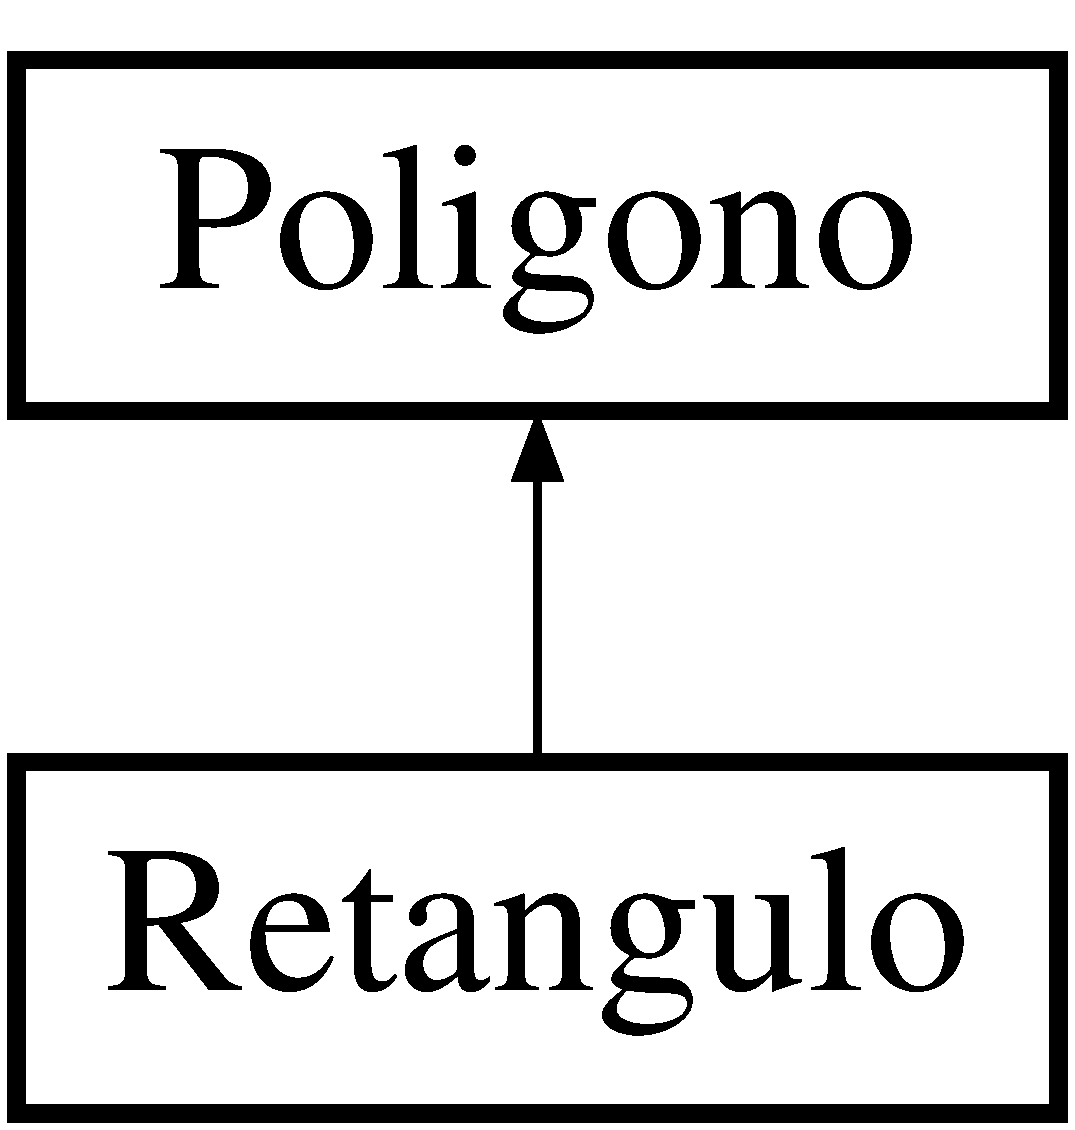
\includegraphics[height=2.000000cm]{class_poligono}
\end{center}
\end{figure}
\subsection*{Public Member Functions}
\begin{DoxyCompactItemize}
\item 
\mbox{\hyperlink{class_poligono_a9311a9a1496878c09c8508b3636e2870}{Poligono}} ()
\begin{DoxyCompactList}\small\item\em Construtor default\+: \end{DoxyCompactList}\item 
\mbox{\Hypertarget{class_poligono_a121937469d43a3b05a821fa14cb51e62}\label{class_poligono_a121937469d43a3b05a821fa14cb51e62}} 
void {\bfseries insert\+Vertice} (\mbox{\hyperlink{class_point}{Point}} p)
\item 
\mbox{\Hypertarget{class_poligono_a5ce6c1bb536a15abea87aeaafcf1f045}\label{class_poligono_a5ce6c1bb536a15abea87aeaafcf1f045}} 
int \mbox{\hyperlink{class_poligono_a5ce6c1bb536a15abea87aeaafcf1f045}{number\+Vertices}} (void)
\begin{DoxyCompactList}\small\item\em Retorna o numero de vértices. \end{DoxyCompactList}\item 
float \mbox{\hyperlink{class_poligono_a9b2abd1369df82e2fa93a145553de590}{calc\+Area}} (void)
\begin{DoxyCompactList}\small\item\em Função que calcula a área do polígono. \end{DoxyCompactList}\item 
\mbox{\Hypertarget{class_poligono_ac8c10a46cd6a60078600085fc136d65e}\label{class_poligono_ac8c10a46cd6a60078600085fc136d65e}} 
void \mbox{\hyperlink{class_poligono_ac8c10a46cd6a60078600085fc136d65e}{translate}} (float a, float b)
\begin{DoxyCompactList}\small\item\em Função para transladar os vértices do polígono. \end{DoxyCompactList}\item 
void \mbox{\hyperlink{class_poligono_a2f0b4d5f528fa2e474b991a6806c3eef}{rotate}} (float ang, \mbox{\hyperlink{class_point}{Point}} p)
\begin{DoxyCompactList}\small\item\em Função para rotacionar o polígono. \end{DoxyCompactList}\item 
\mbox{\Hypertarget{class_poligono_a1a3d812834a6898c0db3d809d1c9a974}\label{class_poligono_a1a3d812834a6898c0db3d809d1c9a974}} 
void \mbox{\hyperlink{class_poligono_a1a3d812834a6898c0db3d809d1c9a974}{impress}} (void)
\begin{DoxyCompactList}\small\item\em Função que imprime o polígono. \end{DoxyCompactList}\end{DoxyCompactItemize}


\subsection{Constructor \& Destructor Documentation}
\mbox{\Hypertarget{class_poligono_a9311a9a1496878c09c8508b3636e2870}\label{class_poligono_a9311a9a1496878c09c8508b3636e2870}} 
\index{Poligono@{Poligono}!Poligono@{Poligono}}
\index{Poligono@{Poligono}!Poligono@{Poligono}}
\subsubsection{\texorpdfstring{Poligono()}{Poligono()}}
{\footnotesize\ttfamily Poligono\+::\+Poligono (\begin{DoxyParamCaption}{ }\end{DoxyParamCaption})}



Construtor default\+: 

Os 100 vértices do polígono são inicializados com (0,0). O número de vértices, por sua vez, é inicializado com 0. 

\subsection{Member Function Documentation}
\mbox{\Hypertarget{class_poligono_a9b2abd1369df82e2fa93a145553de590}\label{class_poligono_a9b2abd1369df82e2fa93a145553de590}} 
\index{Poligono@{Poligono}!calc\+Area@{calc\+Area}}
\index{calc\+Area@{calc\+Area}!Poligono@{Poligono}}
\subsubsection{\texorpdfstring{calc\+Area()}{calcArea()}}
{\footnotesize\ttfamily float Poligono\+::calc\+Area (\begin{DoxyParamCaption}\item[{void}]{ }\end{DoxyParamCaption})}



Função que calcula a área do polígono. 

A função multiplica e soma todas as diagonais principais e secundárias da matriz e subtrai a soma das diagonais principais pela das diagonais secundárias. O resultado divide é dividido por 2. \mbox{\Hypertarget{class_poligono_a2f0b4d5f528fa2e474b991a6806c3eef}\label{class_poligono_a2f0b4d5f528fa2e474b991a6806c3eef}} 
\index{Poligono@{Poligono}!rotate@{rotate}}
\index{rotate@{rotate}!Poligono@{Poligono}}
\subsubsection{\texorpdfstring{rotate()}{rotate()}}
{\footnotesize\ttfamily void Poligono\+::rotate (\begin{DoxyParamCaption}\item[{float}]{ang,  }\item[{\mbox{\hyperlink{class_point}{Point}}}]{p }\end{DoxyParamCaption})}



Função para rotacionar o polígono. 

A função move os pontos para o ponto de rotação, monta a matriz de translação e então os pontos voltam para a posição original já rotacionados 

The documentation for this class was generated from the following files\+:\begin{DoxyCompactItemize}
\item 
poligono.\+h\item 
poligono.\+cpp\end{DoxyCompactItemize}

\hypertarget{class_retangulo}{}\section{Retangulo Class Reference}
\label{class_retangulo}\index{Retangulo@{Retangulo}}
Inheritance diagram for Retangulo\+:\begin{figure}[H]
\begin{center}
\leavevmode
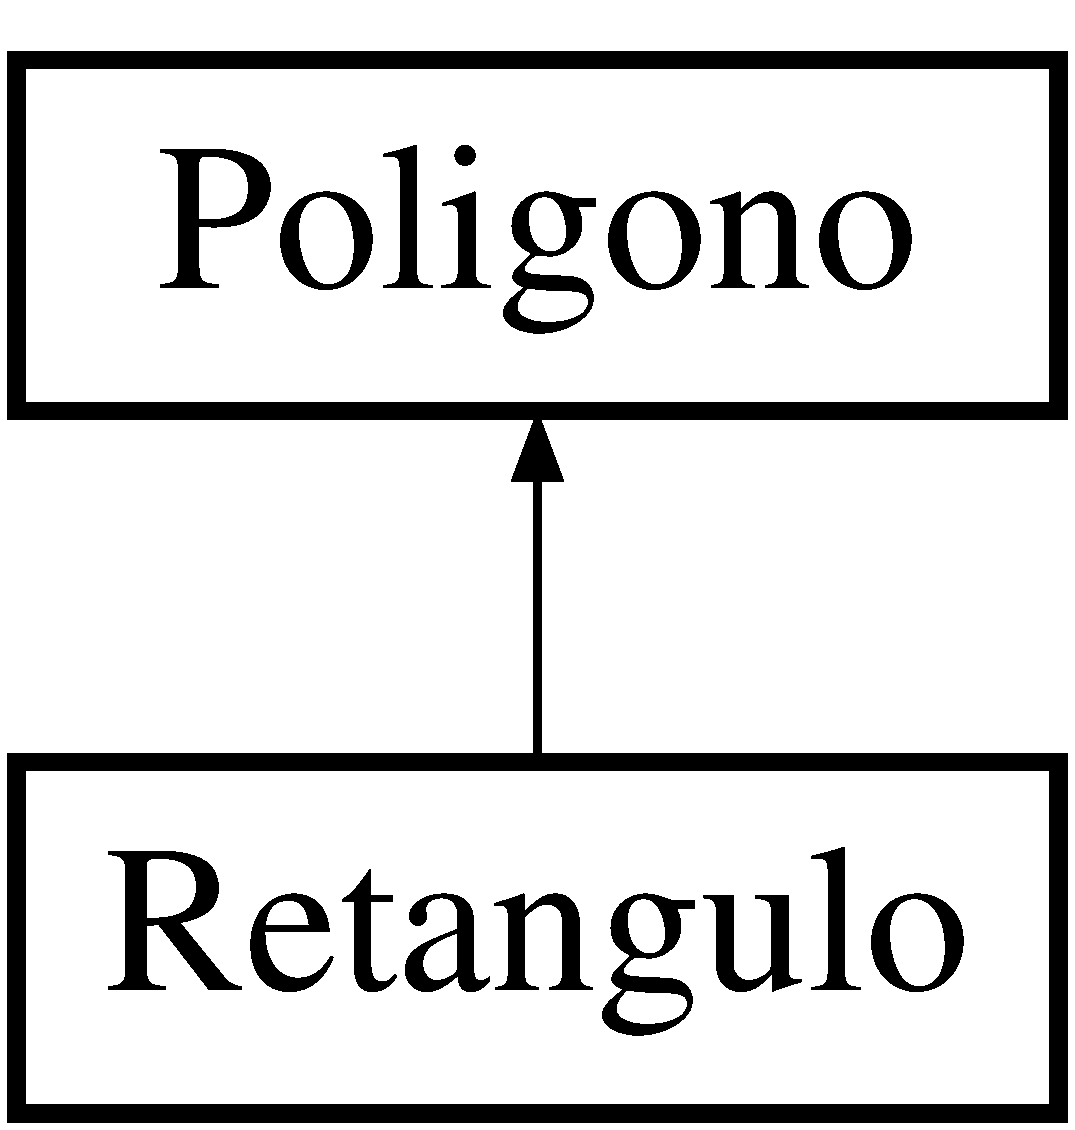
\includegraphics[height=2.000000cm]{class_retangulo}
\end{center}
\end{figure}
\subsection*{Public Member Functions}
\begin{DoxyCompactItemize}
\item 
\mbox{\Hypertarget{class_retangulo_ac971a3083d7f3b268acb5b9373a82c36}\label{class_retangulo_ac971a3083d7f3b268acb5b9373a82c36}} 
{\bfseries Retangulo} (int xc, int yc, int larg, int alt, int fill)
\item 
\mbox{\Hypertarget{class_retangulo_ac088dd6d3f4f3d3f80363a868c2e74f1}\label{class_retangulo_ac088dd6d3f4f3d3f80363a868c2e74f1}} 
void {\bfseries draw} (\mbox{\hyperlink{class_screen}{Screen}} \&t)
\end{DoxyCompactItemize}


The documentation for this class was generated from the following files\+:\begin{DoxyCompactItemize}
\item 
retangulo.\+h\item 
retangulo.\+cpp\end{DoxyCompactItemize}

%--- End generated contents ---

% Index
\backmatter
\newpage
\phantomsection
\clearemptydoublepage
\addcontentsline{toc}{chapter}{Index}
\printindex

\end{document}
